\chapter{Different Approaches for Solving the Drift-Diffusion Equation on Metric Graphs using PINNs}

In this chapter we present different approaches of using a physics informed neural network to solve a set of drift-diffusion equations defined in a given metric graph to given initial and boundary conditions. These approaches will differ in their approach of learning of the used neural networks. In \cref{ch3:sec1}, we discuss a approach in which the drift-diffusion equations on all edges are considered simultaneously in the learning phase. That is, we combine the drift-diffusion equations on all edges of the graph and the associated initial and boundary conditions through a cleverly defined cost function and focus only on solving this single resulting cost function in the learning phase. In \cref{ch3:sec2}, we discuss an approach similar to the idea in \cite{JagtapKharazmiKarniadakis:2020}, where we define a cost function for each edge of the graph, optimize them one by one, store certain relevant data for the interconnection for each edge, and repeat this process several times. Thus, we have as many cost functions as edges of the graph, but in the learning phase they are minimized several times in succession. Nevertheless, in both approaches the same residual network is used for each edge, the approaches only differ in the cost function of the learning method, in which the corresponding neural network and the initial and boundary conditions enter in different ways, and the course of the learning phase, simultaneously or periodically. Furthermore, we use different types and topologies of neural networks for these two approaches. We perform numerical experiments for each combination of PINN approach and neural network and compare the solutions with those generated by the FEM presented in \cref{ch2}. We are particularly interested in the accuracy and efficiency of the different approaches so that we can determine a superior method for solving the differential equation. Finally, in \cref{ch3:sec3}, we compare the performance of a PINN with explicitly calculated derivatives used inside the Hamiltonian, and thus in the corresponding residual network and cost function, with that of a PINN that uses automatic differentiation for this purpose, in order to demonstrate the capabilities of \lstinline!TensorFlow!. \\
In order to compare all the results of all numerical experiments, the set of drift-diffusion equations is considered on the same metric graph $\Gamma$ under the same initial and boundary conditions in each experiment. The graph $\Gamma = (\mathcal{V}, \mathcal{E})$ given by the following adjacency matrix: 
\begin{equation*}
    A^{\Gamma} = 
    \begin{blockarray}{ccccccc}
        v_1 & v_2 & v_3 & v_4 & v_5 & v_6 \\
        \begin{block}{(cccccc)c}
            0 & 0 & 1 & 0 & 0 & 0 & v_1 \\
            0 & 0 & 1 & 0 & 0 & 0 & v_2 \\
            0 & 0 & 0 & 1 & 0 & 0 & v_3 \\
            0 & 0 & 0 & 0 & 1 & 1 & v_4 \\
            0 & 0 & 0 & 0 & 0 & 0 & v_5 \\
            0 & 0 & 0 & 0 & 0 & 0 & v_6 \\
        \end{block}
    \end{blockarray}
\end{equation*}
The graph $\Gamma$ consists of $6$ vertices $\mathcal{V} = \{ v_i \}_{i = 1,\ldots, 6}$ and $5$ edges $\mathcal{E} = \{ e_i \}_{i = 1,\ldots, 5}$  and is of course directed since $A^{\Gamma}$ is not symmetric. The graph $\Gamma$ is illustrated in \cref{fig7}. 
\begin{figure}[H]
    \begin{center}
        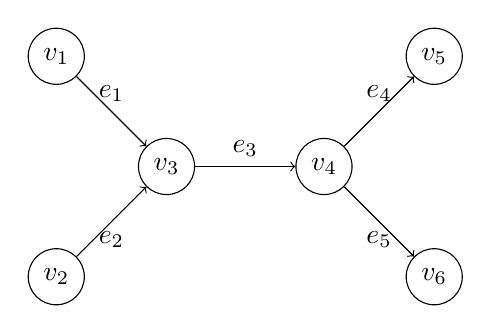
\begin{tikzpicture}
            % vertices
            \node[shape=circle,draw=black] (v1) at (-2.4,1.4) {$v_1$};
            \node[shape=circle,draw=black] (v5) at (2.4,1.4) {$v_5$};
            \node[shape=circle,draw=black] (v3) at (-1,0) {$v_3$};
            \node[shape=circle,draw=black] (v4) at (1,0) {$v_4$};
            \node[shape=circle,draw=black] (v2) at (-2.4,-1.4) {$v_2$};
            \node[shape=circle,draw=black] (v6) at (2.4,-1.4) {$v_6$};
            
            % edges
            \path [->](v1) edge node[above] {$e_1$} (v3);
            \path [->](v2) edge node[below] {$e_2$} (v3);
            \path [->](v3) edge node[above] {$e_3$} (v4);
            \path [->](v4) edge node[above] {$e_4$} (v5);
            \path [->](v4) edge node[below] {$e_5$} (v6);
        \end{tikzpicture}
    \end{center}
    \caption{Will come soon \ldots}
    \label{fig7}
\end{figure}
As we can see, the vertices $v_1$, $v_2$, $v_5$ and $v_6$ are exterior vertices and the vertices $v_3$ and $v_4$ are interior vertices. We further assume that the graph $\Gamma$ is equilateral (see \cref{metric graph equilateral}) with $\ell = 1$. \\
We consider on each individual edge $e \in \mathcal{E}$ the drift-diffusion equation given by \cref{Drift-Diffusion-equation} for $x \in [0,1]$ and on the time interval $t \in (0, 10)$, where we set $\varepsilon = 0.01$, the mobility is given by $f(\rho_e(t,x)) = \rho_e (t,x)(1-\rho_e (t,x))$ and we assume that $\partial_x V_b (t,x) = 1$ for all $(t,x) \in (0, 10) \times [0,1]$ holds. On the exterior vertices $\mathcal{V}_{\mathcal{D}} = \{v_1, v_2, v_5, v_6 \}$, we have for flux boundary conditions, \cref{eq:Dirichlet_conditions}, constant influx rates which are specified for $v_1$ by $\alpha_{v_1}(t) = 0.9$ and $\beta_{v_1}(t) = 0$, for $v_2$ by $\alpha_{v_2}(t) = 0.3$ and $\beta_{v_2}(t) = 0$, for $v_5$ by $\alpha_{v_5}(t) = 0$ and $\beta_{v_5}(t) = 0.8$ and for $v_6$ by $\alpha_{v_6}(t) = 0$ and $\beta_{v_6}(t) = 0.1$. 



The numerical experiments are implemented in the toolbox \lstinline!Manopt.jl!. They were run on a Lenovo ThinkPad L490, 64 bit Windows system, 1.8 Ghz Intel Core i7-8565U, 32 GB RAM, with Julia 1.5.2.

\section{One Neural Network for all edges}
\label{ch3:sec1}

In this section we construct, in some sense, a global cost function, which is used to modify the weights and biases of a neural network appropriately by minimizing it in the learning phase. In the following we denote this cost function by $\Phi_\theta$, where $\theta$ only refers to the set of trainable parameters of the used neural network and does not obtain any information about the used type of neural network or the topology of the used neural network. The idea of this approach in this section is that in the learning phase the drift-diffusion equations on all edges and all initial and boundary conditions are considered at once such that all edges are seen as being merged together and thus the problem of approximating the solution of the set of drift-diffusion equations on a metric graph is treated as a whole. Therefore, we construct only one cost function $\Phi_\theta$, which consists of several misfit terms, as in \cref{MSE PINN}, by incorporating the mean-squared-error of a residual network as well as a number of misfit terms which enforce the initial and boundary conditions at a set of collocation points. Of course, we want to exploit the special structure of the domain given by the metric graph for the construction of this cost function $\Phi_\theta$. We note that we construct the cost function $\Phi_\theta$ for the general case and do not adopt the parameters with respect to the previously mentioned graph, since this approach can of course also be applied to any metric graph. \\
Let's start with the easy part first, the definition of the residual network, which returns us a residual in the cost function $\Phi_\theta$ for the neural network to be learned. From now on, we denote the surrogate network by $\rho_{\theta_e}$, which is supposed to approximate the solution $\rho_e$ of \cref{eq:Hamiltonian} on an individual edge $e \in \mathcal{E}$. Of course, $\rho_{\theta_e}$ receives the same input values $ \left( t, x \right) \in  \left( 0, T \right) \times [0, \ell_e]$ as $\rho_e$ and also returns a real-valued number. Here $\theta_e$ denotes the set of all weights and biases that are involved in the approximation of $\rho_e$ on an individual edge $e \in \mathcal{E}$, and $\theta_e$ also contains no information about the used type of neural network or the topology of the used neural network. If we insert the surrogate network $\rho_{\theta_e} \left( t,x \right)$ into the right-hand side of \cref{eq:Hamiltonian}, we obtain as a residual network for each individual edge $e \in \mathcal{E}$
\begin{equation}
    \label{Drift-Diffusion residual network}
    r_{\theta_e} \left( t,x \right)=\partial_t \rho_{\theta_e} \left( t,x \right) - \partial_x   \left(  \varepsilon \partial_x  \rho_{\theta_e} \left( t,x \right) - f \left( \rho_{\theta_e} \left( t,x \right) \right) \partial_x V \left( t,x \right) \right).
\end{equation}
Using \cref{Drift-Diffusion residual network} we form the residual misfit term for each individual edge $e \in \mathcal{E}$ via
\begin{equation} 
    \label{misfit:residual}
    \phi_{e,r}  \left( X_e \right) \coloneqq \frac{1}{n_e} \sum_{i=1}^{n_e} r_{\theta_e}  \left( x_e^i, t_e^i \right)^2,
\end{equation} 
where $X_e = \{ \left( t_e^i, x_e^i \right)\}_{i=1}^{n_e} \subset \left( 0, T \right) \times [0, \ell_e]$ is a set of time-space collocation points that are drawn randomly or chosen equidistantly. \\
To enforce the Kirchhoff-Neumann conditions, \cref{eq:Kirchhoff_Neumann_condition}, we define the following misfit term for each interior vertex $v \in \mathcal{V}_\mathcal{K}$ 
\begin{equation} 
    \label{misfit:Kirchhoff}
    \phi_{v,K}  \left( X_{v,b} \right) \coloneqq \frac{1}{n_b} \sum_{i=1}^{n_b}  \left( \sum_{e \in \mathcal{E}_v}  \left( - \varepsilon \partial_x \rho_{\theta_e}  \left( t_{v,b}^i, v \right) + f \left( \rho_{\theta_e}  \left( t_{v,b}^i, v \right) \right) \partial_x V_e \left( t_{v,b}^i, v \right) \right) \, n_e  \left( v \right) \right)^2, 
\end{equation} 
where $X_{v,b} = \{t_{v,b}^i\}_{i=1}^{n_b} \subset \left( 0,T \right)$ is a set of time snapshots where the Kirchhoff-Neumann conditions are enforced. We note that the derivatives are taken into the outgoing direction. \\
In order to enforce the continuity in the interior vertices $\mathcal{V}_\mathcal{K}$, required by \cref{continuous on vertices}, we introduce two different misfit terms to accomplish this. In the numerical experiments, we draw attention to which of the two misfit terms is used. The first misfit term is defined for each interior vertex $v \in \mathcal{V}_\mathcal{K}$ by 
\begin{equation} 
    \label{misfit:continuity}
    \phi_{v,c}  \left( X_{v,b} \right) \coloneqq \frac{1}{n_b} \sum_{e \in \mathcal{E}_v} \sum_{i=1}^{n_b} \left(  \rho_{\theta_e}  \left( t_{v,b}^i, v \right) - \rho_{v}^i \right)^2,
\end{equation} 
with $X_{v,b} = \{t_{v,b}^i\}_{i=1}^{n_b}$ as introduced before. Here, we introduce for each interior vertex $v \in \mathcal{V}_\mathcal{K}$ some additional trainable parameters $\{\rho_{v}^i\}_{i=1}^{n_b}$, that are appended to the set of weights and biases $\theta$ and which are also trained by minimizing the resulting cost function $\Phi_\theta$. The other misfit is defined for each interior vertex $v \in \mathcal{V}_\mathcal{K}$ by 
\begin{equation} 
    \label{misfit:continuity:average}
    \phi_{v,c}  \left( X_{v,b} \right) \coloneqq \frac{1}{n_b}  \sum_{i=1}^{n_b} \left( \sum_{e \in \mathcal{E}_v} \left( \rho_{\theta_e}  \left( t_{v,b}^i, v \right) - \frac{1}{\abs{\mathcal{E}_v}} \sum_{e \in \mathcal{E}_v} \rho_{\theta_e}  \left( t_{v,b}^i, v \right) \right) \right)^2.
\end{equation}
Here, on average over all time collocation points $\{t_{v,b}^i\}_{i=1}^{n_b}$, the value $\rho_{\theta_e}  \left( t_{v,b}^i, v \right)$ of each edge $e \in \mathcal{E}_v$ should be equal to the average of all edges connected to this interior vertex $v \in \mathcal{V}_\mathcal{K}$. Both misfit terms have their numerical advantages and disadvantages. The misfit term defined by \cref{misfit:continuity} is not so complex, from which can follow that the derivatives with respect to the trainable parameters in the optimization method is easier to compute, but therefore it introduces just as much trainable parameters as collocation points to the set of trainable parameters. No further trainable parameters need to be defined for the misfit term given by \cref{misfit:continuity:average}, but it is more complex for that. \\
We enforce the flux boundary conditions for each exterior vertex $v \in \mathcal{V}_\mathcal{D}$, \cref{eq:Dirichlet_conditions} by defining the following misfit term  
\begin{align} 
    \label{misfit:Dirichlet}
    \phi_{v,D}  \left( X_{v,b} \right) \coloneqq & \frac{1}{n_b} \sum_{i=1}^{n_b} \bigg( \sum_{e \in \mathcal{E}_v} \left(- \varepsilon \partial_x \rho_{\theta_e}  \left( t_{v,b}^i, v \right) + f\left(\rho_{\theta_e}  \left( t_{v,b}^i, v \right)\right) \partial_x V_e\left( t_{v,b}^i, v \right) \right) n_e  \left( v \right) + \\
    & \alpha_v \left( t_{v,b}^i \right)  \left( 1- \rho_{\theta_e}  \left( t_{v,b}^i, v \right) \right) - \beta_v \left( t_{v,b}^i \right) \rho_{\theta_e}  \left( t_{v,b}^i, v \right) \bigg)^2
\end{align}
with $X_{v,b} = \{t_{v,b}^i\}_{i=1}^{n_b}$ as introduced before. \\
To enforce the initial conditions for each edge $e \in \mathcal{E}$, \cref{eq:initial_conditions}, we define the following misfit term  
\begin{equation} 
    \label{misfit:initial}
    \phi_{e,0}  \left( X_{e,0} \right) \coloneqq \frac{1}{n_0} \sum_{i=1}^{n_0}  \left( \rho_{\theta_e}  \left( 0,x_{e,0}^i \right) - \rho_{e,0} \left( x_{e,0}^i \right) \right)^2, 
\end{equation} 
where $X_{e,0} = \{x_{e,0}^i\}_{i=1}^{n_0} \subset [0, \ell_e]$ is a set of collocation points along $t=0$. \\ 

We average each of the above mentioned misfit terms over all units where these terms hold and sum up the averages to form $\Phi_\theta$:
\begin{align} 
    \label{eq:loss:1}
    \Phi_{\theta} \left( X_{data} \right) & =  \frac{1}{\abs{\mathcal{V}_\mathcal{D}}} \sum_{v \in \mathcal{V}_\mathcal{D}} \phi_{v,D} \left( X_{v,b} \right) + \frac{1}{\abs{\mathcal{V}_\mathcal{K}}} \sum_{v \in \mathcal{V}_\mathcal{K}}  \left(  \phi_{v,K}  \left( X_{v,b} \right) + \phi_{v,c} \left( X_{v,b} \right)  \right) + \\
    & \quad + \frac{1}{\abs{\mathcal{E}}} \sum_{e \in \mathcal{E}}  \left(  \phi_{e,r}  \left( X_{e,r} \right) + \phi_{e,0}  \left( X_{e,0} \right)  \right), 
\end{align}
where $X_{data}$ represents the union of the different collocation points $X_e$, $X_{v,b}$ and $X_{e,0}$. 

Next we perform numerical experiments with different types of neural networks for this approach specified by the cost function given by \cref{eq:loss:1}. So far we have not specified what type of neural network with which topology we use for $\rho_{\theta_e}(t, x)$, i.e. to approximate the solution of \cref{Drift-Diffusion-equation} on an individual edge under the given initial and vertex conditions. Of course, we have an infinite freedom of choice, the only constraints being the dimension of the input $(x,t) \in \mathbb{R}^2$, the dimension of the output $\rho_{\theta_e}(t, x) \in \mathbb{R}$ and the differentiability of the corresponding neural network up to order two (due to $\partial_{xx} \rho_{\theta_e}(t,x)$ appears in \cref{Drift-Diffusion-equation}). \\
Since we have to find an approximation for each edge $e \in \mathcal{E}$ and the approximations are simply summed up in the cost function $\Phi_{\theta}$, it is obvious to use a single network for the approximation of the solution of \cref{Drift-Diffusion-equation} on one individual edge, which results in the fact that we use as many neural networks as we have edges of the graph $\Gamma$. In this case, $\theta_e$ describes the trainable parameters of a single neural network and $\theta$ is the union of all trainable parameters of all networks. Thus, during training, all trainable parameters in $\theta$ are modified when the cost function $\Phi_{\theta}$ is minimized, and therefore consider the corresponding optimization methods$\theta$ as the optimization variable. A set of neural networks offers the possibility to choose different training parameters such as collocation points but also different hyperparameters such as activation functions or the topology of the corresponding neural network. One can use a deep neural network for an edge for which the solution can have a complex structure, while a shallow neural network can be used on the edges with relatively simple and smooth solutions. In this work, however, we will not cover such a case due to the effort of finding the best set of collocation points or the best hyperparameters, but we use the same type of neural network with the same topology for each edge. \\

% Noch die richtigen Hyperparameter hinzufügen
For the first numerical experiment, we use for $\rho_{\theta_e}(x, t)$ an feed-forward neural network, denoted by $fnn_{\theta_e}(x, t)$, with $L$-layers and $n_0 = 2$, $n_L = 1$ for each edge $e \in \mathcal{E}$, which is defined by 
\begin{gather}
    \label{one_for_each}
    fnn_{\theta_e} \colon \mathbb{R}^2 \to \mathbb{R} \\
    \\
    fnn_{\theta_e}(x, t) = \sigma_L(W^L \sigma_{L-1}(W^{L-1}\sigma_{L-2}(\cdots \sigma_{1}(W^{1}x^0 +b^1) \cdots) + b^{L-1}) + b^{L}) 
\end{gather}
where $x^0 = (t, x)^{\mathrm{T}} \in (0, T) \times [0, \ell_e] \subset \mathbb{R}^2$ and $\theta_e = \left\{ \left\{ W^l \right\}_{l = 1, \ldots, L}, \left\{ b^l \right\}_{l = 1, \ldots, L} \right\}$. The total set of all trainable parameters for this PINN approach is therefore $\theta = \bigcup_{e \in \mathcal{E}} \ \theta_e$. Feed-forward neural networks have already been used in various PINN setups, so this choice can be considered reasonable.  \\
For the second numerical experiment, we use a neural network for $\rho_{\theta_e}(x, t)$, which is defined by the following architecture and the following forward propagation
\begin{gather}
    \label{Resnet1}
    R_{\theta_e} \colon \mathbb{R}^2 \to \mathbb{R} \\
    \\
    R_{\theta_e}(t,x) = \frac{1}{2} {x^0}^{\mathrm{T}} A x^0 + w^{\mathrm{T}} x^{L} + c^{\mathrm{T}} x^0
\end{gather}
with
\begin{gather}
    \label{Resnet2}
    x^1 = \sigma_1(W^1 x^{0} + b^1) \in \mathbb{R}^m \\
    \\
    x^l = x^{l-1} + h \cdot \sigma_l(W^l x^{l-1} + b^l) \in \mathbb{R}^m \quad \text{for} \quad l = 2, \ldots, L, 
\end{gather}
where $x^0 = (t, x)^{\mathrm{T}} \in (0, T) \times [0, \ell_e] \subset \mathbb{R}^2$, $h > 0$ is called stepsize and is a hyperparameter and $A \in \mathbb{R}^{2 \times 2}$, $w \in \mathbb{R}^m$, $c \in \mathbb{R}^2$ are also trainable parameters, i.e. $\theta_e = \left\{ \left\{ W^l \right\}_{l = 1, \ldots, L}, \left\{ b^l \right\}_{l = 1, \ldots, L}, A, w, c \right\}$ and $\theta = \bigcup_{e \in \mathcal{E}} \ \theta_e$. The idea of using this type of neural network originates from \cite{RuthottoOsherLiNurbekyanFung2020}, in which high-dimensional mean field games and mean field control models are approximately solved by combining Lagrangian and Eulerian viewpoints and by using a tailored neural network parameterization for the potential of the solution, which can be understood as a density, to avoid any spatial discretisation. The neural network given by  is also called residual network and abbreviated with ResNet, \cite{HeZhangRenSun:2015}. We refer to it only as ResNet to avoid confusion with the residual network of a PINN. ResNets have been successful in a wide range of machine learning tasks and have been found to be trainable even for many layers. By interpreting \cref{Resnet2} as a forward Euler discretization of an initial value problem, the continuous limit of a ResNet is amenable to mathematical analysis, \cite[p.~6]{RuthottoOsherLiNurbekyanFung2020}. \\

For the third numerical experiment, we use a completely different approach of utilize a neural network to approximate the solutions of the set of drift-diffusion equations. We use one single feed-forward neural network with $L \in \mathbb{N}$ layers for the approximation of the solution of \cref{Drift-Diffusion-equation} under the given initial and boundary conditions on all edges of the graph $\Gamma$, i.e. this network returns for a point $(t,x) \in \mathcal{R}^2$ the values $\rho_{\theta_{e_i}}(x, t)$ for all edges $\mathcal{E} = \left\{ e_i \right\}_{i = 1, \ldots, E}$, where $E = \abs{\mathcal{E}}$. We define this neural network as follows
\begin{gather}
    \label{one_for_all}
    \mathfrak{FNN}_{\theta} \colon \mathbb{R}^2 \to \mathbb{R}^E \\
    \\
    \mathfrak{FNN}_{\theta}(x, t) = \sigma_L(W^L \sigma_{L-1}(W^{L-1}\sigma_{L-2}(\cdots \sigma_{1}(W^{1}x^0 +b^1) \cdots) + b^{L-1}) + b^{L}) \in \mathbb{R}^E
\end{gather}
the approximation values are given by 
\begin{equation*}
    \rho_{\theta_{e_i}}(x, t) = \left[ \mathfrak{FNN}_{\theta}(x, t) \right]_i \in \mathbb{R},
\end{equation*}
i.e. the $i$-th entry of the networks output $\mathfrak{FNN}_{\theta}(x, t) \in \mathbb{R}^E$ is the approximation of the solution on the $i$-th edge. In this case, the trainable parameters consist only of the weights and biases of this single neural network, i.e. $\theta = \left\{ \left\{ W^l \right\}_{l = 1, \ldots, L}, \left\{ b^l \right\}_{l = 1, \ldots, L} \right\}$, as indicated by the index $\theta$ in $\mathfrak{FNN}_{\theta}$. \\
The use of a single neural network is motivated by the hope that the neurons in the hidden layers will learn the structure of the entire graph and the resulting communication of the edges via the vertices, i.e. that all interactions inside the graph will be taken into account by the neurons. Furthermore, we hope that the computational cost is reduced as only the weights and biases of this single network need to be trained, provided it can be shown that the depth and width of the network is not too large. The fact that the network generates the output for all edges at the same time is also an advantage, as in an implementation only the execution of one network is necessary instead of several. However, we point out that this approach only makes sense if the graph is equilateral, see \cref{graph_assumptions}, because then the same collocation points $X_e = \{ \left( t_e^i, x_e^i \right)\}_{i=1}^{n_e}$ and $X_{e,0} = \{x_{e,0}^i\}_{i=1}^{n_0}$ can be used for the misfit terms given by \cref{misfit:residual} and \cref{misfit:initial} for all edges $e \in \mathcal{E}$.


% Erklärung der Knoten v in den misfit termen!






% Kollokationspunkte 

We note that, as mentioned in \cref{ch1:sec4}, all derivatives of surrogate models with respect to the input parameters are computed with automatic differentiation provided by \lstinline!Tensorflow! via the method \lstinline!tf.GradientTape!. 


For the minimization of the cost function $\Phi_{\theta}$, we first use a variant of the gradient descent method, in which the direction is given by the Adam optimizer from the module \lstinline!Keras!, see \cite{Chollet:2015}, which belongs to the package \lstinline!Tensorflow!, see \cite{TensorFlow}. We change for the different types of neural networks the input parameter \lstinline!learning_rate!, which obviously specifies the learning rate of the method, and leave all other input parameters of the Adam optimizer by default. This method stops after 2000 iterations. After that, we use the L-BFGS-B optimizer from the package \lstinline!SciPy!, see \cite{SciPy:2020}, and we set for all networks as parameters in the options \lstinline!maxiter = 5000! which specifies the maximum number of iterations, \lstinline!maxfun = 50000! which specifies the maximum number of function evaluations, \lstinline!maxcor = 50! which specifies the maximum number of stored variable metric corrections used in the L-BFGS approximation of the Hessian of the cost function $\Phi_{\theta}$, \lstinline!maxls = 50! which specifies the maximum number of line search steps per iteration and \lstinline!ftol = 1.0*np.finfo(float).eps! which specifies a parameter in a stopping criterion that aborts the method if the values of the cost function $\Phi_{\theta}$ between two iterates are too small.


\begin{table}[H]\label{tab:one_cost_function}
    \resizebox{\textwidth}{!}{
        \begin{tabular}{l l l l }
            \toprule
            Neural Network given by & One each egde & Resnet & One  \\ 
            \midrule
            Error & $0.15$ & $0.21$ & $0.54$ \\ 
            \midrule
            Time in seconds & $0.15$ & $0.21$ & $0.54$  \\ 
            \midrule
            Number of Iterations & $72$ & $68$ & $72$ \\
            \bottomrule
        \end{tabular}
    }
    \caption{Comparison of different types of neural networks.}
\end{table}
\section{One Neural Network for each edge}
\label{ch3:sec2}

In this section, we present a PINN approach for solving the set of drift-diffusion equations on a metric graph, where a cost function for the approximation of $\rho_e \colon (0,T) \times [0, \ell_e] \to [0, 1]$ is defined for each edge $e \in \mathcal{E}$ of the graph $\Gamma = (\mathcal{V}, \mathcal{E})$, where the included misfit terms are defined in such a way that the solution of the approximation problem on the entire graph is ensured. The idea for this approach is adopted from \cite{JagtapKharazmiKarniadakis:2020}, in which so-called conservative physics-informed neural networks, abbreviated cPINNs, on discrete domains for non-linear conservation laws were presented. In \cite{JagtapKharazmiKarniadakis:2020} the domain on which the relevant conservation law is defined is split into several adjacent subdomains and one neural network is used as a PINN to solve the conservation law in one subdomain. The conservation property is achieved on the whole domain by enforcing the flux continuity in the strong form along the intersections of these subdomains. Apart from the flux continuity condition, an average solution given by two different neural networks is also enforced at the common interface between two sub-domains. The cost function of cPINN is defined for each subdomain, which has a similar structure as the PINN cost function in each subdomain, but these two interface conditions are incorporated by misfit terms. Consequently, one has as many cost functions as subdomains into which one has split the original domain. These cPINN cost functions are then minimized several times in succession with an optimization method, such as SGD, with respect to their learnable parameters dependent on the corresponding subdomain, and certain values, which are needed e.g. for the average solution at the common interface between two sub-domains, are stored. The splitting into several subdomains allows to use neural networks with different architectures for each subdomain to obtain the solution of the same underlying PDE, and also allows to choose different non-learnable hyperparameters such as the type of optimization method for the minimization in the learning phase. Also there is a possibility to train the networks in parallel, i.e., simultaneously, which is very important in terms of achieving computational efficiency. The domain decomposition in the cPINN approach together with the use of an individual neural network for the different subdomains offers as an advantage the possibility for the reduction of the approximation error. \\
We adopt for our approach this idea of splitting the domain into several subdomains and receiving an individual cost function for each subdomain. For this purpose, we associate the individual subdomains with the individual edges of the considered graph, i.e. we construct now a cost function for each edge of the considered graph. These cost functions for all edges are minimized several times in succession, always training only the learnable parameters that are needed to approximate the solution on exactly this edge.\\
We now construct the cost function for the approximation of the solution of \cref{Drift-Diffusion-equation} on a single edge, which we denote by $\hat{e} \in \mathcal{E}$ to distinguish it more easily from the other edges $e \in \mathcal{E} \setminus \{ \hat{e}\}$. In the following, we denote the cost function for an individual edge by $\Phi_{\theta_{\hat{e}}}$, where $\theta_{\hat{e}}$ denotes the learnable parameters which are used for the approximation of $\rho_{\hat{e}}$. Like the cost functions given by \cref{eq:loss:1} and \cref{MSE PINN}, the cost function $\Phi_{\theta_{\hat{e}}}$ consists also of several misfit terms. \\
Since we require that the corresponding neural network approximates the solution of the drift-diffusion equation on the edge e, therefore we incorporate the mean squared error of the residual network given by \cref{Drift-Diffusion residual network}

the term given by Equation 3 into our cost function.  

Two misfit terms always appear the same, term 1 and term 2, where we can simply incorporate equation 1 and equation 2 into the cost function here. 

Each edge is defined by two vertices which it connects and by which it is linked to other edges. When we construct a cost function for an individual edge, both vertices must be checked to see if they are either an interior or an exterior vertex, since it follows that different conditions apply and thus different terms are incorporated into the cost function. 

Fortunately, we can incorporate two terms from Section 2, the term for the residual network and the term for the initial condition. This is because these terms are defined for each edge individually and the average of these terms over all edges is incorporated in the final cost function. Here we do not incorporate the average of all edges into the cost function, but only the term for one edge. This is to ensure that the trained neural network approximates the solution of the equation on this edge and satisfies the initial conditions.  \\

What the interface conditions are in \cite{JagtapKharazmiKarniadakis:2020} are here the vertex conditions that couple the edges at a vertex, i.e., \cref{eq:Kirchhoff_Neumann_condition} and \cref{continuous on vertices} on the interior vertices $\mathcal{V}_\mathcal{K}$ and \cref{eq:Dirichlet_conditions} on the exterior vertices $\mathcal{V}_\mathcal{D}$. 

Each edge is defined by two vertices which it connects and by which it is linked to other edges. When we construct a cost function for an individual edge, both vertices must be checked to see if they are either an interior or an exterior vertex, since it follows that different conditions apply and thus different terms are incorporated into the cost function. 

To enforce the Kirchhoff-Neumann condition on an interior vertex $v \in \mathcal{V}_\mathcal{K}$, \cref{eq:Kirchhoff_Neumann_condition}, we use the misfit term given by \cref{misfit:Kirchhoff}, but we rewrite it, so that it is apparent that only the learnable parameters, which are necessary for the approximation of the solution on the corresponding edge, are trained. The misfit term for an interior vertex $v \in \mathcal{V}_\mathcal{K}$ is given by
\begin{equation} 
    \label{misfit:Kirchhoff.}
    \phi_{v,K}  \left( X_{v,b} \right) \coloneqq \frac{1}{n_b} \sum_{i=1}^{n_b}  \left( \sum_{e\in \mathcal{E}_v} J_e(t,v) n_e (v) \right)^2, 
\end{equation} 
where $X_{v,b} = \{t_{v,b}^i\}_{i=1}^{n_b} \subset \left( 0,T \right)$ is a set of time snapshots where the Kirchhoff-Neumann conditions are enforced. We note that the derivative is taken into the outgoing direction. \\

When a cost function is trained for one edge, in the optimization procedure the learnable parameters of the networks of the other edges are fixed



If we set up a cost function for an individual edge, then we have to check what these vertices are, because consequently different conditions apply and are included in the cost function. 
\begin{equation}
    \label{vertex funcions}
    \phi_{v}(X_{v,b}) = \begin{cases} \phi_{v,K}  \left( X_{v,b} \right) +  \phi_{v,c}  \left( X_{v,b} \right)& \text{if } v \in \mathcal{V}_{\mathcal{K}}, \\ \phi_{v,D}  \left( X_{v,b} \right) & \text{if } v \in \mathcal{V}_{\mathcal{D}}, \end{cases}
\end{equation}


We define for each edge the cost function $e = (v^{o}_e, v^{t}_e) \in \mathcal{E}$
\begin{equation}
    \label{eq:cost:2}
    \phi_{\theta_e} \left( X_{data} \right) \coloneqq \phi_{e,r}  \left( X_e \right) + \phi_{e,0}  \left( X_{e,0} \right) + \phi_{v^{o}_e}(X_{v,b}) + \phi_{v^{t}_e}(X_{v,b})
\end{equation}
\section{Automatic differentiation vs explicit derivatives}
\label{ch3:sec3}

In this section we show how the neural networks used in the previous numerical tests can be explicitly differentiated so that the use of automatic differentiation in a PINN can be omitted. We compare the time to convergence and the computational resources required for a PINN programmed in Python with explicit derivatives with the results previously obtained for a PINN that of course uses automatic differentiation. This aims to show whether an explicit calculation of the derivatives for our problem brings computational advantages with it and whether the performance of a PINN can be improved as a result. \\
Let us first consider the case of the feed-forward neural network. In this work we used two FNNs with different topologies. First, an FNN was used in section 1 for all edges of the graph and then an FNN was used for each individual edge of the graph. We are interested in finding an explicit formula for the gradient of the output used for an individual edge of one of these two neural networks. For this purpose, we first calculate the first-order derivative with respect to a vector of a general FNN $f_{\theta}$ with $L$ layers. In the following, $f_{\theta}(x) \in \mathbb{R}^{n_L}$ denotes the model prediction of this neural network for an input value $x = x^0 \in \mathbb{R}^{n_0}$, which is defined by 
\begin{equation}
    \label{model prediction}
    f_{\theta}(x) = x^{L} = f^{L}_{\theta_L}(x^{L-1}) = \sigma_{L} (W^{L} x^{L-1} + b^{L}) \in \mathbb{R}^{n_L} 
\end{equation}
and 
\begin{equation*}
    x^{l} = \sigma_{l} (W^{l} x^{l-1} + b^{l}) \in \mathbb{R}^{n_l}, 
\end{equation*}
for $0 \leq l \leq L-1$. We are interested in the first order derivative of $f_{\theta} \colon \mathbb{R}^{n_0} \to \mathbb{R}^{n_L}$ with respect to the input value $x = x^0 \in \mathcal{R}^{n_0}$, which can be represented by the Jacobian matrix of $f_{\theta}$
\begin{equation*}
    \frac{\mathrm{d}}{\mathrm{d} \ x} f_{\theta}(x) = \mathrm{}J[f_{\theta}](x)= \begin{pmatrix} \dfrac{\partial f_{\theta}(x)}{\partial x_{1}} & \cdots & \dfrac{\partial f_{\theta}(x)}{\partial x_{n_0}} \end{pmatrix} = \begin{pmatrix} \nabla f_{\theta, 1}(x)^{\mathrm{T}} \\ \vdots \\  \nabla f_{\theta, n_L}(x)^{\mathrm{T}} \end{pmatrix} = \begin{pmatrix} \dfrac{\partial f_{\theta, 1}(x)}{\partial x_{1}} & \cdots & \dfrac{\partial f_{\theta, 1}(x)}{\partial x_{n_0}} \\ \vdots & \ddots & \vdots \\ \dfrac{\partial f_{\theta, n_L}(x)}{\partial x_{1}} & \cdots & \dfrac{\partial f_{\theta, n_L}(x)}{\partial x_{n_0}} \end{pmatrix} 
\end{equation*}
where $f_{\theta, i}(x)$ is the $i$-th component of the output $f_{\theta}(x) \in \mathbb{R}^{n_L}$ and $\nabla f_{\theta, n_L}(x)^{\mathrm{T}}$ is the transpose of the gradient of $f_{\theta, i}(x)$. \\
To calculate the Jacobi matrix of $f_{\theta}$ we use the chain rule several times in order to differentiate the network layer by layer. For that we denote the Jacobian matrix of the activation function $\sigma_{l} \colon \mathbb{R}^{n_l} \to \mathbb{R}^{n_l}$ of the $l$-th layer with respect to the activation $a^l(x^{l-1}) = W^{l} x^{l-1} + b^{l}$ of the $l$-th layer, with
\begin{equation*}
    \frac{\mathrm{d}}{\mathrm{d} \ a^{l}} \ \sigma_{l} (a^l) = D^{l} \in \mathbb{R}^{n_l \times n_l}.
\end{equation*}
We remind that the activation function of a layer is defined component-wise, thus the Jacobian matrix is a diagonal matrix and its diagonal entries are given by
\begin{equation*}
    D_{i, i}^{l} = {\sigma_{l}}^{\prime} (a^{l}(x^{l-1}))_i = {\sigma_{l}}^{\prime} (a^{l}(x^{l-1})_i).
\end{equation*} 
We can now differentiate the network using the chain rule
\begin{align*}
    \frac{\mathrm{d}}{\mathrm{d} \ x} f_{\theta}(x) & = \frac{\mathrm{d}}{\mathrm{d} \ a^{L}} \ \sigma_{L} (a^{L}(x^{L-1})) = \\
    & = D^L \cdot \frac{\mathrm{d}}{\mathrm{d} \ x^{L-1}} \ a^{L}(x^{L-1}) = D^L \cdot \frac{\mathrm{d}}{\mathrm{d} \ x^{L-1}} \ (W^{L} x^{L-1} + b^{L}) = \\
    & = D^L \cdot W^L \cdot \frac{\mathrm{d}}{\mathrm{d} \ a^{L_1}} \ \sigma_{L-1} (a^{L-1}(x^{L-2})) = \\
    & = \ldots = \\
    & = D^L \cdot W^L \cdot D^{L-1} \cdot \ldots \cdot W^2 \cdot D^1 \cdot \frac{\mathrm{d}}{\mathrm{d} \ x^{0}} \ (W^{1} x^{0} + b^{1}) = \\
    & = D^L \cdot W^L \cdot D^{L-1} \cdot \ldots \cdot W^2 \cdot D^1 \cdot W^{1} \in \mathbb{R}^{n_L \times n_0}.
\end{align*}

Let us return to our case where an FNN rho approximates the solution of the drift-diffusion equation on an edge. In the following we use the vector z, where its first component is the time and the second component is the position on an edge. The gradient is due to equation 3 and equation 4 given by 
\begin{equation}
    \begin{split}
        \nabla_{z}  \ \rho_{\theta_e}(z) & = \left(\nabla_{z} \rho_{\theta_e}(z)^{\mathrm{T}} \right)^{\mathrm{T}} = \left(D^L \cdot W^L \cdot D^{L-1} \cdot \ldots \cdot W^2 \cdot D^1 \cdot W^{1} \right)^{\mathrm{T}} = \\
        & = {W^{1}}^{\mathrm{T}} \cdot D^{1} \cdot {W^{2}}^{\mathrm{T}} \cdot \ldots \cdot {W^{L}}^{\mathrm{T}}  \cdot  D^{L}. 
    \end{split}
\end{equation}
The partial derivatives can be obtained by 
\begin{equation*}
    \begin{split}
        \partial_t \rho_{\theta_e}(t,x) = \nabla_{z} \ \rho_{\theta_e}(z)_1 \quad & \text{and} \quad \partial_x \rho_{\theta_e}(t,x) = \nabla_{z} \ \rho_{\theta_e}(z)_2 \\
        \partial_t \rho_{\theta_e}(t,x) = {\nabla_{z} \ \rho_{\theta_e}(z)}^{\mathrm{T}} \begin{pmatrix} 1 \\ 0 \end{pmatrix} \quad & \text{and} \quad \partial_x \rho_{\theta_e}(t,x) = {\nabla_{z} \ \rho_{\theta_e}(z)}^{\mathrm{T}} \begin{pmatrix} 0 \\ 1 \end{pmatrix}.
    \end{split}
\end{equation*}


To compute the gradient in a computer program, one proceeds similarly to backpropagation by first evaluating the network at a point, i.e. propagating information forwards through the network, storing relevant values, and then propagating the so-called error backwards through the network by applying the chain rule from the last layer to the first layer in reverse. The following iterative computation can be used for that purpose
\begin{align*}
    \delta^{L} & = {W^{L}}^{\mathrm{T}} \mathrm{diag}({\sigma_{L}}^{\prime}(W^{L} a^{L-1}(s) + b^{L})) = {W^{L}}^{\mathrm{T}} D^{L} \in \mathbb{R}^{n_{L-1}} \\
    \delta^{l} & = {W^{l}}^{\mathrm{T}} D^{l} \cdot \, \delta^{[l+1]} \, \cdot \, \ldots \,  \cdot \, \delta^{L} \in \mathbb{R}^{n_{l-1}} \quad \text{for} \quad l = 2, \ldots, L-1
\end{align*}


We set 
% Tensor + n-Modul-Produkt
\begin{equation*}
    H^{l} = \mathrm{diag}({\sigma_{l}}^{\prime \prime}(W^{l} a^{l-1}(s) + b^{l})) \in \mathbb{R}^{n_l \times n_l}, \quad (H^{l})_{i, i} = {\sigma_{l}}^{\prime \prime} (z_{i}^{l})
\end{equation*}

\begin{align*}
    \nabla^{2} f_{\theta}(s) & = \eta^{[1]} \in \mathbb{R}^{2 \times 2} \\
    \eta^{[1]} & = {W^{[1]}}^{\mathrm{T}} \left( \mathrm{diag}(H^{[1]} \delta^{[2]}) + D^{[1]} \eta^{[2]} D^{[1]} \right) W^{[1]} \\
    & \vdots \\
    \eta^{l} & = {W^{l}}^{\mathrm{T}} \left( \mathrm{diag}(H^{l} \delta^{[l+1]}) + D^{l} \eta^{[l+1]} D^{l} \right) W^{l} \in \mathbb{R}^{n_{l-1} \times n_{l-1}} \\
    & \vdots \\
    \eta^{L} & = {W^{L}}^{\mathrm{T}} H^{L} W^{L} \in \mathbb{R}^{n_{L-1} \times n_{L-1}}
\end{align*} 


\begin{algorithm}[H]
    \caption{Computation of the gradient and a Hessian of an L-layer feed-forward neural network.}
    \begin{algorithmic}[1]
        \State \textbf{Input:} vector $z^0 \in \mathbb{R}^{n_0}$; trainable parameters $\theta = (\{ W^l \}_{l = 1, \ldots, L}, \{ b^l \}_{l = 1, \ldots, L})$ with $W^l \in \mathbb{R}^{n_l \times n_{l-1}}$ and $b^l \in \mathbb{R}^{n_l}$ for $l = 1, \ldots, L$, where $n_L = 1$; activation functions $\{ b^l \}_{l = 1, \ldots, L}$ and their first order derivative up to order 2 of a FNN $f$
        \For{$ l = 1, \ldots, L$}
            \State Set $z^l = \sigma_l(W^l z^{l-1} + b^l)$
        \EndFor
        \State Set $\delta^{L} = {W^{L}}^{\mathrm{T}} \mathrm{diag}({\sigma_{L}}^{\prime}(W^{L} z^{L-1} + b^{L}))$.
        \State Set $\eta^{L}$.
        \For{$ l = 1, \ldots, L-1$}
            \State Set $\delta^{l} = {W^{l}}^{\mathrm{T}} \mathrm{diag}({\sigma_{l}}^{\prime}(W^{l} z^{l-1} + b^{l})) \cdot \delta^{l+1}$.
            \State Set $\eta^{l}$.
        \EndFor
        \State \textbf{Input:} $z^L$, $\delta^1$, $\eta^1$.
    \end{algorithmic}
\end{algorithm}




  






We note that for $A \in \mathbb{R}^{m \times n}$, $b \in \mathbb{R}^{m}$, $c, d \in \mathbb{R}^{n}$

\begin{align*}
    d \, \odot \, c &= c \, \odot \, d \in \mathbb{R}^{n} \\
    \mathrm{diag}(b) \, \cdot \, A &= b \, \odot \, A \in \mathbb{R}^{m \times n} \\
    A \, \cdot \, \mathrm{diag}(c) &= A \, \odot \, c^{\mathrm{T}} \in \mathbb{R}^{m \times n} \\
    \mathrm{diag}(b) \, \cdot \, A \, \cdot \, \mathrm{diag}(c) &= b \, \odot \, A \, \odot \, c^{\mathrm{T}} \in \mathbb{R}^{m \times n} \\
    \mathrm{diag}(c) \, \cdot \, d &= c \, \odot \, d \in \mathbb{R}^{n} \\
    c^{\mathrm{T}} \, \cdot \, \mathrm{diag}(d) &= c^{\mathrm{T}} \, \odot \, d^{\mathrm{T}} \in \mathbb{R}^{1 \times n} \\
\end{align*}







\subsection{Backpropagation in ResNet}



where $W^{[1]} \in \mathbb{R}^{m \times 2}$ and $b^{[1]} \in \mathbb{R}^{m}$.

\begin{equation*}
    a^{l}(x) = a^{l-1}(x) + h \, \sigma_{l} (z^{l}(x)) = a^{l-1}(x) + h \, \sigma_{l} (W^{l} a^{l-1}(x) + b^{l}) \in \mathbb{R}^{m}, 
\end{equation*}

for $l = 2, \ldots, L$, where $W^{[2]}, \ldots, W^{L} \in \mathbb{R}^{m \times m}$ and $b^{[2]}, \ldots, b^{L} \in \mathbb{R}^{m}$.

\begin{equation*}
    f_{\theta}(x) = f_{\theta}(s) = w^{\mathrm{T}} a^{L}(s) + \frac{1}{2} s^{\mathrm{T}} A s + c^{\mathrm{T}} s 
\end{equation*}

where $s = (x)^{\mathrm{T}} \in \mathbb{R}^{2}$, $w \in \mathbb{R}^{m}$, $A \in \mathbb{R}^{2 \times 2}$ and $c \in \mathbb{R}^2$.

\textbf{Gradient:}

\begin{equation*}
    \nabla_s f_{\theta}(s) = \nabla_s a^{L}(s) \, w + A s + c
\end{equation*}

We set

\begin{equation*}
    D^{l} = \mathrm{diag} \left( \frac{\mathrm{d}}{\mathrm{d}z^{l}} \sigma_{l} (z^{l}) \right) \in \mathbb{R}^{m \times m}, \quad D_{i, i}^{l} = {\sigma_{l}}^{\prime} (z_{i}^{l})
\end{equation*}

\begin{align*}
    \nabla_s a^{L}(s) \, w & = \delta^{[1]}  \\
    \delta^{[1]} & = {W^{[1]}}^{\mathrm{T}} D^{[1]} \, \delta^{[2]} \\
    \delta^{[2]} & = \delta^{[3]} + h \, {W^{[2]}}^{\mathrm{T}} D^{[2]} \, \delta^{[3]} \\
    &\vdots\\
    \delta^{l} & = \delta^{[l+1]} + h \, {W^{l}}^{\mathrm{T}} D^{l} \, \delta^{[l+1]} \\
    &\vdots\\
    \delta^{L-1} & = \delta^{L} + h \, {W^{L-1}}^{\mathrm{T}} D^{L-1} \, \delta^{L} \\
    \delta^{L} & = w + h \, {W^{L}}^{\mathrm{T}} D^{L} \, w
\end{align*}


\textbf{Hessian:}

First my derivation:

Ruthotto computes the Laplacian of the potential model with respect to the spatial variable $x$. For this he uses the trace of the Hessian matrix of our model $f_{\theta}(s)$, i.e. 

\begin{align*}
    \Delta_x f_{\theta}(s) & = \mathrm{tr}(E^{\mathrm{T}} \, \nabla^{2}_s f_{\theta}(s) \, E) = \\
    & = \mathrm{tr}(E^{\mathrm{T}} \, (\nabla^{2}_s a^{L}(s) \, w + A) \, E) = \\
    & = \mathrm{tr}(E^{\mathrm{T}} \, \nabla^{2}_s a^{L}(s) \, w \, E) + \mathrm{tr}(E^{\mathrm{T}} \,  A \, E) = \\
    & = \Delta_x (a^{L}(s) \, w) + \mathrm{tr}(E^{\mathrm{T}} \,  A \, E)
\end{align*}

where the columns of $E \in \mathbb{R}^{(d+1) \times d}$ are given by the first $d$ standard basis vectors in $R^{d+1}$ so that only the second derivative of the spatial coordinates $x \in \mathbb{R}^d$ is computed. In our case we use $E = (1, 0)^{\mathrm{T}} \in \mathbb{R}^{2}$. \\
Ruthotto sets

\begin{align*}
    \Delta_x (a^{L}(s) \, w) & = t^{[0]} + h \, \sum^{L}_{l=1} t^{l} = \mathrm{tr}(\eta^{[0]}) + h \, \sum^{L}_{l=1} \mathrm{tr}(\eta^{l}) = \\
    & = \mathrm{tr} \left( \eta^{[0]} + h \, \sum^{L}_{l=1} \eta^{l} \right) = \mathrm{tr} \left( \nabla^{2}_x a^{L}(s) \, w \right)
\end{align*}

\begin{equation*}
    \partial_{xx} a^{L}(s) w = \nabla^{2}_x a^{L}(s) w = E^{\mathrm{T}} \, \nabla^{2}_s a^{L}(s) \, w \, E = \eta^{[0]} + h \, \sum^{L}_{l=1} \eta^{l}
\end{equation*}

where 

\begin{equation*}
    \eta^{[0]} = E^T {W^{[1]}}^{\mathrm{T}} \mathrm{diag}({\sigma_{[1]}}^{\prime \prime}(W^{[1]} s + b^{[1]}) \odot \delta^{[2]}) W^{[1]} E
\end{equation*}

\begin{equation*}
    \eta^{l} = {J^{l-1}}^{\mathrm{T}} {W^{l}}^{\mathrm{T}} \mathrm{diag}({\sigma_{l}}^{\prime \prime}(W^{l} a^{l-1}(s) + b^{l}) \odot \delta^{[l+1]}) W^{l} J^{l-1}
\end{equation*}

where 

\begin{equation*}
    J^{l-1} = J_x(a^{l-1}(s)) = \left( \frac{\mathrm{d}}{\mathrm{d} x} a^{l-1}_1(s), \ldots, \frac{\mathrm{d}}{\mathrm{d} x} a^{l-1}_m(s) \right)^{\mathrm{T}} \in \mathbb{R}^{m}
\end{equation*}


Now to the Hessian as it has been implemented: 

\begin{align*}
    \eta^{[1]} & = h \, {W^{[1]}}^{\mathrm{T}} \mathrm{diag} \left( H^{[1]} \delta^{[2]} \right) W^{[1]} + \\
    & \quad + \left( I + h \, {W^{[1]}}^{\mathrm{T}} D^{[1]} \right) \, \left( \left( I + h \, {W^{[1]}}^{\mathrm{T}} D^{[1]} \right) \, \eta^{[2]} \right)^{\mathrm{T}} \\ 
    &\vdots\\
    \eta^{l} & = h \, {W^{l}}^{\mathrm{T}} \mathrm{diag} \left( H^{l} \delta^{[l+1]} \right) W^{l} + \\
    & \quad + \left( I + h \, {W^{l}}^{\mathrm{T}} D^{l} \right) \, \left( \left( I + h \, {W^{l}}^{\mathrm{T}} D^{l} \right) \, \eta^{[l+1]} \right)^{\mathrm{T}} \\ 
    \eta^{l} & = h \, {W^{l}}^{\mathrm{T}} \mathrm{diag} \left( H^{l} \delta^{[l+1]} \right) W^{l} + \\
    & \quad + \left( I + h \, {W^{l}}^{\mathrm{T}} D^{l} \right) \, \eta^{[l+1]}  \left( I + h \,  D^{l} {W^{l}} \right) \\ 
    &\vdots\\
    \eta^{L-1} & = h \, {W^{L-1}}^{\mathrm{T}} \mathrm{diag} \left( H^{L-1} \delta^{L} \right) W^{L-1} + \\
    & \quad + \left( I + h \, {W^{L-1}}^{\mathrm{T}} D^{L-1} \right) \, \left( \left( I + h \, {W^{L-1}}^{\mathrm{T}} D^{L-1} \right) \, \eta^{L} \right)^{\mathrm{T}} \\
    \eta^{L} &  = h \, {W^{L}}^{\mathrm{T}} \mathrm{diag}(H^{L} w) W^{L} 
\end{align*}

